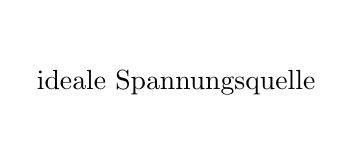
\begin{tikzpicture}[x=1mm,y=1mm]\draw[draw=none] (-10,-7) rectangle (+10,+7); \node[draw=none,align=center] {ideale Spannungsquelle};\end{tikzpicture} & {\begin{tikzpicture} \draw(0,1.5) to[european voltage source, name=V] (0,0); \draw[white] (-1.3,1.5) to[] (-1.35,1.59); \varrmore{V}{$U_0$}; \end{tikzpicture}} \\
\hline
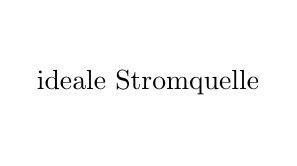
\begin{tikzpicture}[x=1mm,y=1mm]\draw[draw=none] (-10,-7) rectangle (+10,+7); \node[draw=none,align=center] {ideale Stromquelle};\end{tikzpicture} & {\begin{tikzpicture} \draw(0,0) to[european current source, name=A] (0,1.5); \iarrmore{A}{$I_0$}; \end{tikzpicture}} \\
\hline
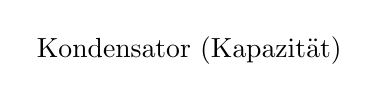
\begin{tikzpicture}[x=1mm,y=1mm]\draw[draw=none] (-10,-2) rectangle (+10,+2); \node[draw=none,align=center] {Kondensator (Kapazität)};\end{tikzpicture} & {\begin{tikzpicture} \draw(0,0) to[C] (1.5,0); \draw[white] (-0.1,-.10) to[] (0,0.5);\end{tikzpicture}} \\
\hline
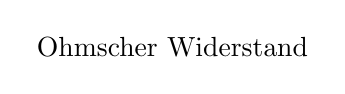
\begin{tikzpicture}[x=1mm,y=1mm]\draw[draw=none] (-10,-2) rectangle (+10,+2); \node[draw=none,align=center] {Ohmscher Widerstand};\end{tikzpicture}& {\begin{tikzpicture} \draw(0,0) to[R] (1.5,0);  \draw[white] (-0.1,-.10) to[] (0,0.35); \end{tikzpicture}} \\
\hline
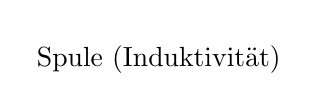
\begin{tikzpicture}[x=1mm,y=1mm]\draw[draw=none] (-10,-1) rectangle (+10,+4); \node[draw=none,align=center] {Spule (Induktivität)};\end{tikzpicture}& {\begin{tikzpicture} \draw(0,0) to[L] (1.5,0); \draw[white] (-0.1,-.10) to[] (0,0.35); \end{tikzpicture}}